101. \begin{figure}[ht!]
\center{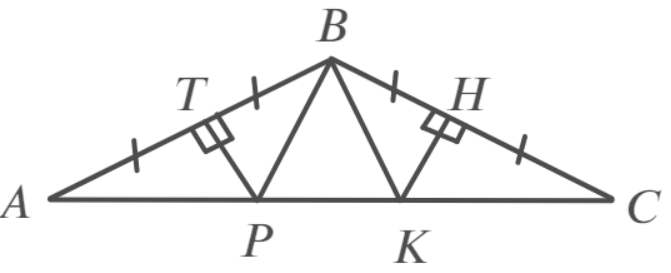
\includegraphics[scale=0.35]{g101.png}}
\end{figure}\\
В треугольниках $ABP$ и $CBK$ совпадают высота и медиана, значит они равнобедренные и $AP=BP,\ CK=BK.$ Так как $ABC$ тоже равнобедренный, $\angle A=\angle C=(180^\circ-120^\circ):2=30^\circ,$ значит $\angle ABP=\angle CBK=30^\circ,\ \angle PBK=120^\circ-30^\circ-30^\circ=60^\circ,\ \angle BPK=\angle BKP=180^\circ-120^\circ=60^\circ,$ поэтому треугольник $BKP$ равносторонний и $BP=BK=KP.$ Таким образом, $AP+PK+KC=AC,\ 3PK=AC,\ PK=21:3=7$см.\\
